%%\title{BEAMBEAM}
%  Changed by: Chris ISELIN, 23-Jan-1997 
%  Changed by: Hans Grote,   25-Sep-2002 
%  Changed by: Stefan Sorge, 2007 

\section{BEAMBEAM: Beam-beam Interaction}
 
The command BEAMBEAM may be inserted in a beam line to simulate a
beam-beam interaction point:  
 
\begin{verbatim}
label: BEAMBEAM, SIGX = real, SIGY = real,
                 XMA = real, YMA = real, CHARGE = real
                 BBSHAPE = int, WIDTH = real, BBDIR = int;
\end{verbatim}

The beam-beam interaction is represented by a four-dimensional
interaction with a thin element, i.e. horizontal and vertical non-linear kicks.
The code for this element has been contributed by J.M. Veuillen (1987)
and extended by S. Sorge (2007).  
 
\begin{itemize}
   \item SIGX:
     The horizontal extent of the opposite beam (default: 1 m).
     Meaning depends on parameter BBSHAPE.
   \item SIGY:
     The vertical extent of the opposite beam (default: 1 m).
     Meaning depends on parameter BBSHAPE.
   \item XMA:
     The horizontal displacement of the opposite beam with respect to
     the ideal orbit (default: 0 m).
   \item YMA:
     The vertical displacement of the opposite beam with respect to
     the ideal orbit (default: 0 m).
   \item CHARGE:
     The charge of particles in the opposite beam in elementary charges. 
     It is set by default CHARGE=1. So, if you want to describe collisions 
     between beams containing the same particles having a charge different 
     from 1, you have to set CHARGE explicitly in BEAM and 
     in BEAMBEAM. 
   \item BBSHAPE: The parameter to choose the radial density shape of the 
     opposite beam (default: 1)
     \begin{itemize}
       \item  BBSHAPE=1: Gaussian shape (default), SIGX/SIGY: standard deviation in 
         vertical/horizontal direction.
	\item  BBSHAPE=2: \href{beambeam_n_trapez.jpg}{trapezoidal shape}, 
          SIGX/SIGY: half width of density profile,
          i.e. distance from the centre to half edge region with linear decrease of 
          density in horizontal/vertical direction. Still only circular opposite beam 
          possible, i.e. in the calculations 
          SIGX'=SIGY'=(SIGX+SIGY)/2 is used, if SIGX and SIGY have
          different values 
%\\\href{beambeam_n_trapez.jpg}{
\\
\includegraphics[width=400px]{Introduction/beambeam_n_trapez.jpg}
\label{fig:beambeam_n_trapez}
%%\includegraphics{beambeam_n_trapez.jpg}}
\\
        \item  BBSHAPE=3: \href{beambeam_n_hollowparabol.jpg}{hollow-parabolic shape}, 
          SIGX/SIGY: distance from the centre 
          to the maximum of the parabolic density profile in vertical/horizontal 
          direction. Still only circular opposite beam possible, 
          i.e. in the calculations 
          SIGX'=SIGY'=(SIGX+SIGY)/2 is used, if SIGX and SIGY have different values 
\\
%\\\href{beambeam_n_hollowparabol.jpg}
%\begin{figure}[p]
\includegraphics[width=420px]{Introduction/beambeam_n_hollowparabol.jpg}
\label{fig:beambeam_n_hollowparabol}
%%\includegraphics{beambeam_n_hollowparabol.jpg} 
%\end{figure}
\\
     \end{itemize}
     
     The restriction to circular opposite beams in the cases BBSHAPE=2,3 
     appears to be sufficient, because such beam profiles are more important 
     for the description of the interaction between the particle beam and 
     an electron beam of an electron cooler, which are usually circular. 
     
   \item  WIDTH: The relative extent of the edge region, absolute value is given by 
     WIDTH*SIGX and WIDTH*SIGY vertical and horizontal direction, respectively. 
     For 
     \begin{itemize}
        \item  BBSHAPE=1, WIDTH is meaningless and will be ignored.
	\item  BBSHAPE=2, WIDTH denotes the full width of the edge region in units of 
          SIGX (or SIGX' and SIGY', respectively, if SIGX and SIGY are not equal), i.e. 
          if WIDTH=0.01 and SIGX=5 mm, the edge  region has a full width of 0.05
          mm. It must be WIDTH \textless   2.0.
	\item  BBSHAPE=3, WIDTH denotes the full width at half maximum of the parabolic 
          density profile in units of SIGX (or SIGX' and SIGY', respectively, if SIGX 
          SIGY are not equal. It must be WIDTH \textless   SQRT(2.0).
     \end{itemize} 
   \item  BBDIR: The parameter to choose the direction of motion of the 
     opposite beam relative to the beam considered. It determines 
     the sign of the Lorenz force between the both beams (default: -1): 
     \begin{itemize}
        \item  BBDIR=-1: Beams move in the opposite direction as in a collider. 
          Therefore, the Lorenz force enhances the beam-beam interaction. 
	\item  BBDIR=0: Opposite beam does not move, Lorenz force is neglected 
	\item  BBDIR=1: Beams move in the same direction as in an electron cooler. 
          So, the Lorenz force reduces the beam-beam interaction. 
     \end{itemize}
     Note:  
     \begin{itemize}  
        \item  The particles in the beam considered may have a momentum deviation 
          given by DELTAP defined in the TRACK command. 
	\item  The opposite beam is assumed to have the velocity according to the 
          unperturbed energy o the particles in the beam considered. 
          So, only the direction of motion can be chosen. 
	\item  In the case of motion in the opposite direction (BBDIR=-1), 
          the time of interaction between the beams is given by 
          tau = length/(2*beta*c\_light), where length is the length of a bunch in the 
          opposite beam. In the case of motion in the same direction 
          (BBDIR=1) as in an electron cooler, this time 
          is given by tau = length/(beta*c\_light), where length is the length of 
          the cooler. So, the factor 1/2 is inserted only for BBDIR=-1 to calculate 
          correct results. 
     \end{itemize} 
\end{itemize}


A beam-beam element requires the particle energy
(\href{beam.html#energy}{ENERGY})
and the particle charge
(\href{beam.html#charge}{CHARGE})
as well as the number of particles per bunch 
(\href{beam.html#npart}{NPART})
to be set by a \href{beam.html}{BEAM} command
before any calculations are performed.


Examples of a four-dimensional beam-beam element definition:
 
Collider regime example:
\begin{verbatim}
beam,   particle = positron, npart = 1.e12, energy = 50.0;
bb:     beambeam, sigx = 1.e-3, sigy = 5.e-4, charge = 1.;
\end{verbatim}


Electron cooler example: 
\begin{verbatim}
gamma0 = 1.032;                           ! relativistic factors
beta0 = sqrt(1.0-1.0/gamm0/gamma0);

i_e = 0.2;                                ! electron current
re_cool = 0.01;                           ! electron beam radius
l_cool = 5.0;                             ! cooling length
nelect = i_e*l_cool/beta0/clight/qelect;  ! electron number in e-cooler

beam, particle = antiproton, gamma = gamma0, npart = nelect; 
bb_ecool: beambeam, sigx = re_cool, sigy = re_cool, bbshape = 2, 
                    width = 0.01, charge = -1, bbdir = 1;
\end{verbatim}

For the definition of the LHC head-on and parasitic beam-beam elements see 
 \href{../control/foot.html#macro}{beam-beam element examples}.

 %\href{http://www.cern.ch/Hans.Grote/hansg_sign.html}{hansg}, ssorge,  July 13, 2007
